\documentclass{report}
\usepackage{amsmath}
\usepackage{ngerman}
\usepackage[hidelinks]{hyperref}
\usepackage[numbered]{bookmark}
\usepackage{pgfplots}
\usepackage{listings}
\usepackage{color}

\usetikzlibrary{positioning,matrix,arrows.meta,automata}

\pgfplotsset{compat=1.18}
\tracinglostchars=2

\definecolor{dkgreen}{rgb}{0,0.6,0}
\definecolor{gray}{rgb}{0.5,0.5,0.5}
\definecolor{mauve}{rgb}{0.58,0,0.82}

\lstset{
    frame=tb,
    language=Java,
    aboveskip=3mm,
    belowskip=3mm,
    showstringspaces=false,
    columns=flexible,
    basicstyle={\footnotesize\ttfamily},
    numbers=left,
    stepnumber=1,
    numberstyle=\tiny\color{gray},
    keywordstyle=\color{blue},
    commentstyle=\color{dkgreen},
    stringstyle=\color{mauve},
    breaklines=true,
    breakatwhitespace=false,
    tabsize=4
}

\title{\textbf{Informatik-Abitur}}
\author{Tim Teichmann}
\date{\today}

\begin{document}
\maketitle
\tableofcontents

\chapter{Datenstrukturen}
\begin{flushleft}   
    Datenstrukturen speichern Daten, damit später ohne Probleme auf diese Daten zugegriffen werden kann.
    Man nennt sie Daten\textbf{\textit{strukturen}}, da die Daten, die gespeichert werden auf eine bestimmte Art und Weise angeordnet (strukturiert) werden.
\end{flushleft}

\section{Statisch}
\begin{flushleft}
    Statische Datenstrukturen sind -- wie der Name schon sagt -- bestimmt.
    Sie sind relativ fest angeordnet und können schlecht bis gar nicht verändert werden.
\end{flushleft}

\subsection{Array}
\begin{flushleft}
    Arrays sind im Prinzip Listen, die eine feste Größe haben.
    Sie speichern Elemente eines Typs.
    Das bedeutet, dass ein einzelnes Array nicht dafür gedacht ist Integer und Strings zu speichern. \\
    Um Arrays vernünftig zu verstehen sieht man hier ein Beispiel für ein Array, das Integer speichert:
\end{flushleft}

\begin{center}
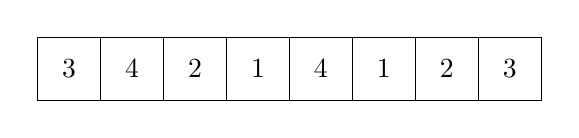
\begin{tikzpicture}
    \matrix (A) [matrix of nodes, nodes={draw, minimum size=8mm},column sep=-\pgflinewidth]{
        3 & 4 & 2 & 1 & 4 & 1 & 2 & 3 \\
    };
\end{tikzpicture}
\end{center}

\begin{flushleft}
    Arrays weisen jedem Element, das sie speichern einen \textit{Index} zu.
    Indices (Mehrzahl eines Index) starten in der Regel bei $0$.
    Das erste Element des Beispiel-Arrays hat den Wert $3$ und liegt beim Index $0$.
    Hier ein Beispiel zur Erstellung und Nutzung eines Arrays in Java.
\end{flushleft}

\begin{center}  
\begin{lstlisting}
// Array.java

// Unser Beispiel-Array erstellen
int[] array = {3,4,2,1,4,1,2,3};

// Die Laenge unseres Beispiel-Arrays abrufen
int arrLen = array.length;

// Den Wert des ersten Elements (3) in die Variable firstElem speichern
int firstElem = array[0];

// Ein Array erstellen, das vier mal den Wert 0 speichert
int[4] array1;
\end{lstlisting}
\end{center}

\section{Dynamisch}
\begin{flushleft}   
    Dynamische Datenstrukturen sind -- vorallem im Vergleich zu statischen Datenstrukturen -- agil.
    Es ist sehr viel leichter Elemente zu entfernen oder hinzuzufügen, da die Größe von dynamischen Datenstrukturen nicht fest ist.
\end{flushleft}

\subsection{Queue}
\subsubsection{Einführung}

\begin{flushleft}   
    Queue bedeutet übersetzt Warteschlange oder Schlange.
    Genau nach diesem Prinzip funktioniert auch eine Queue. \\
    Ein Mensch stellt sich in eine Schlange hinter andere Menschen.
    Vor ihm werden viele Leute aufgerufen, bis er dran kommt.
    Jede Person in der Warteschlange wird nacheinander abgearbeitet.
    Die erste Person, die sich anstellt, wird auch als erstes aufgerufen. \\
    Das nennt man auch \textit{First-In-First-Out} (\textit{FIFO}) Prinzip.
    Hier ein Bild zu der Erklärung:
\end{flushleft}

\begin{center}
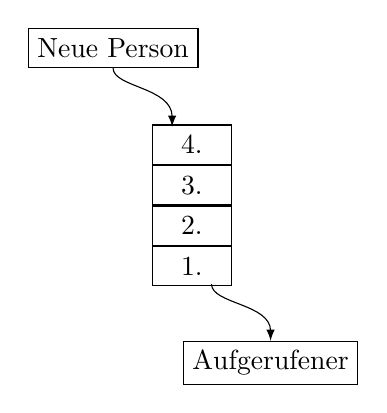
\begin{tikzpicture}[draw,minimum width=1cm,minimum height=0.5cm]
    \node[draw] (in) at (-1,2) {\text{Neue Person}};
    \node[draw] (out) at (1,-2) {\text{Aufgerufener}};
    \matrix (queue)[matrix of nodes,nodes={draw, nodes={draw}}]{
         4. \\ 3. \\ 2. \\ 1. \\
     };

    \draw[-latex] (0.25,-1) .. controls (0.25,-1.25) and (1,-1.25) .. (out.north);
    \draw[-latex] (in.south) .. controls (-1,1.5) and (-0.25,1.5) .. (-0.25,1);
\end{tikzpicture}
\end{center}

\begin{flushleft}
    Das Aufrufen einer Person, entfernt diese aus der Queue.
    Dieser Prozess wird auch \textit{dequeue} genannt.
    Wenn sich eine neue Person anstellt, wird sie der Queue hinzugefügt.
    Das nennt man \textit{enqueue}. \\
    Weitere typische Operationen einer Queue sind:
    \begin{enumerate}
        \item {
                Das erste Element einer Queue aufrufen mit \textit{front}
            }
        \item {
                Prüfen ob die Queue leer ist mit \textit{isEmpty}
            }
    \end{enumerate}
    Eine allgemeine Queue würde also so aussehen:
\end{flushleft}

\begin{center}
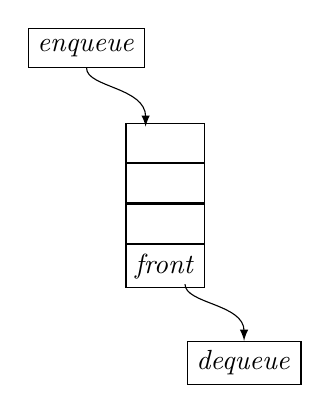
\begin{tikzpicture}[draw,minimum width=1cm,minimum height=0.5cm]
    \node[draw] (in) at (-1,2) {\textit{enqueue}};
    \node[draw] (out) at (1,-2) {\textit{dequeue}};
    \matrix (queue)[matrix of nodes,nodes={draw, nodes={draw}},nodes in empty cells]{
        \\ \\ \\ \textit{front} \\
    };

    \draw[-latex] (0.25,-1) .. controls (0.25,-1.25) and (1,-1.25) .. (out.north);
    \draw[-latex] (in.south) .. controls (-1,1.5) and (-0.25,1.5) .. (-0.25,1);
\end{tikzpicture}
\end{center}

\begin{flushleft}
    Im Abitur wird eine Queue als Java-Klasse vorgegeben. \\
    \href{https://raw.githubusercontent.com/tim-tm/articles/refs/heads/main/informatik-notes/code/Queue.java}{\textit{Abiturvorgabe: Queue}}
\end{flushleft}

\subsubsection{Anwendung}
\begin{flushleft}
    Für Queues gibt es meistens immer ähnliche Aufgaben: \\
    Einfache Queues:
\end{flushleft}

\begin{center}   
\begin{lstlisting}
// Erstellt eine Queue von Strings
Queue<String> queue = new Queue<>();

// Fuegt der Queue eine neues Element mit dem Wert "Hallo" hinzu
queue.enqueue("Hallo");

// Gibt das erste Element der Queue ("Hallo") in der Konsole aus
System.out.println(queue.front());

// Entfernt das erste Element ("Hallo") aus der Queue
queue.dequeue();
\end{lstlisting}
\href{https://raw.githubusercontent.com/tim-tm/articles/refs/heads/main/informatik-notes/code/Queue_Beispiel1.java}{\textit{Unkommentierter Code}} \\
\end{center}

\begin{flushleft}
    Queues mit eigenen Klassen:
\end{flushleft}

\begin{center}
\begin{lstlisting}
// Unsere eigene Klasse um Koordinaten zu speichern
class Koordinate {
    int x;
    int y;
}

// Erstellt eine Queue von Koordinaten
Queue<Koordinate> queue = new Queue<>();

// Wir moechten eine neue Koordinate hinzufuegen
// 1. Die Koordinate erstellen
Koordinate coord = new Koordinate();

// 2. Werte fuer x und y setzen
coord.x = 100;
coord.y = 150;

// 3. Die Koordinate der Queue hinzufuegen
queue.enqueue(coord);

// Die erste Koordinate ausgeben
// 1. Die Koordinate aus der Queue holen
Koordinate koord = queue.front();

// 2. X-Wert der Koordinate ausgeben
System.out.println(koord.x);

// 3. Y-Wert der Koordinate ausgeben
System.out.println(koord.y);

// Erste Koordinate (x=100, y=150) aus der Queue entfernen
queue.dequeue();
\end{lstlisting}
\href{https://raw.githubusercontent.com/tim-tm/articles/refs/heads/main/informatik-notes/code/Queue_Beispiel2.java}{\textit{Unkommentierter Code}} \\
\end{center}

\begin{flushleft}
    Bei diesem Beispiel fällt vorallem auf, dass plötzlich viel mehr Schritte benötigt werden um ein Element hinzuzufügen.
    Das kann vereinfacht werden indem man der Klasse einen \textit{Konstruktur} gibt.
    Der \textit{Konstruktor} wird ausgeführt wenn man ein neues Objekt der Klasse erstellt.
\end{flushleft}

\begin{center}
\begin{lstlisting}
// Unsere eigene Klasse um Koordinaten zu speichern
class Koordinate {
    int x;
    int y;
    
    /** 
        * Diese besondere Methode (Konstruktur) wird aufgerufen, wenn wir new Koordinate() ausfuehren.
        * Unsere Variablen x und y sollen zu den neuen Werten, also unseren Parametern xNeu und yNeu gesetzt werden.
        * Achtung: Der Name des Konstruktors muss genau mit dem Namen der Klasse uebereinstimmen.
        */
    public Koordinate(int xNeu, int yNeu) {
        x = xNeu;
        y = yNeu;
    }
}

// Erstellt eine Queue von Koordinaten
Queue<Koordinate> queue = new Queue<>();

// Wir moechten eine neue Koordinate hinzufuegen
// 1. Die Koordinate erstellen
// Anstatt unsere Werte fuer x und y erst nach dem Erstellen einzutragen, packen wir diese jetzt einfach direkt in die Klammern, wenn wir unsere Koordinate erstellen.
// Das funktioniert nur, weil wir in der Definition unserer Klasse einen Konstruktor erstellt haben.
Koordinate coord = new Koordinate(100, 150);

// 2. Schritt faellt weg

// 3. (jetzt 2.) Die Koordinate der Queue hinzufuegen
queue.enqueue(coord);

// Ausgeben und entfernen bleibt gleich
\end{lstlisting}
\href{https://raw.githubusercontent.com/tim-tm/articles/refs/heads/main/informatik-notes/code/Queue_Beispiel3.java}{\textit{Unkommentierter Code}} \\
\end{center}

\begin{flushleft}
    Dadurch, dass wir einen Konstruktor erstellt haben, sparen wir uns jedes mal wenn wir ein Objekt erstellen zwei Zeilen code. \\
    Kompliziertere Aufgaben mit Queues:
\end{flushleft}

\begin{center}
\begin{lstlisting}
/*
 * 1. 
 *      Die Aufgabenstellung sagt uns, dass es bereits eine Queue namens queue gibt, diese speichert Strings.
 *      Wir sollen jedes Element dieser Queue entfernen und ausgeben lassen.
 */

// Die Schleife wird durchlaufen, solange es noch Elemente in der Queue gibt.
// Also solange sie nicht leer ist (!isEmpty).
while (!queue.isEmpty()) {
    // Das erste Element der Queue in der Variable s speichern
    String s = queue.front();

    // Die Variable s, also das erste Element der Queue ausgeben lassen
    System.out.println(s);

    // Das erste Element (hier: s) aus der Queue entfernen
    // Ohne diesen Schritt wuerde die Schleife unendlich lange das erste Element ausgeben
    queue.dequeue();
}
\end{lstlisting}
\href{https://raw.githubusercontent.com/tim-tm/articles/refs/heads/main/informatik-notes/code/Queue_Beispiel4.java}{\textit{Unkommentierter Code}} \\
\end{center}

\subsection{Stack}
\subsubsection{Einführung}

\begin{flushleft}
    Die deutsche Übersetzung für ein Stack ist: Stapel.
    Das sind Stacks auch, ein Stapel auf den man Dinge legen, oder von dem man Dinge nehmen kann.
    Stacks funktionieren nach dem \textit{Last-In-First-Out} (\textit{LIFO}) Prinzip.
    Man kann also immer nur das letzte Element, was auf den Stapel gelegt wurde wieder vom Stapel nehmen.
    Typische Operationen sind:
    \begin{enumerate}
        \item {
                \textit{push} - Elemente hinzufügen
            }
        \item {
                \textit{pop} - Elemente entfernen
            }
        \item {
                \textit{top} - Auf das oberste Element zugreifen
            }
        \item {
                \textit{isEmpty} - Prüfen ob der Stack leer ist
            }
    \end{enumerate}
    So kann man sich einen Stack vorstellen:
\end{flushleft}

\begin{center}
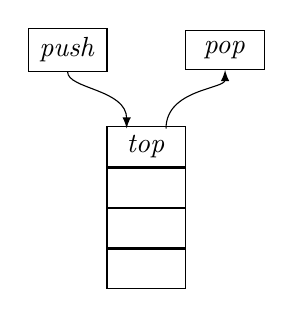
\begin{tikzpicture}[draw, minimum width=1cm, minimum height=0.5cm]
    \node[draw] (in) at (-1,2) {\textit{push}};
    \node[draw] (out) at (1,2) {\textit{pop}};
    \matrix (queue)[matrix of nodes, nodes={draw, nodes={draw}}, nodes in empty cells]
    {
        \textit{top} \\ \\ \\ \\
    };

    \draw[-latex] (0.25,1) .. controls (0.25,1.5) and (1,1.5) .. (out.south);
    \draw[-latex] (in.south) .. controls (-1, 1.5) and (-0.25,1.5) .. (-0.25,1);
\end{tikzpicture}
\end{center}

\begin{flushleft}
    Wie bei der Queue wird im Abitur eine Java Stack Klasse vorgegeben:
    \href{https://raw.githubusercontent.com/tim-tm/articles/refs/heads/main/informatik-notes/code/Stack.java}{\textit{Abiturvorgabe: Stack}} \\
\end{flushleft}

\subsubsection{Anwendung}

\chapter{Automatentheorie}
\begin{flushleft}
    Die Automatentheorie befasst sich mit formalen Sprachen und Grammatiken.
    Es geht hauptsächlich darum diese Sprachen durch Automaten zu verarbeiten.
\end{flushleft}

\section{Endliche Automaten}
\subsection{Definition}
\begin{flushleft}
    Ein endlicher Automat wird durch so einen 5er-Tupel definiert:
    \begin{align}
        A=(\Sigma,Q,\delta,q_0,F)
    \end{align}
    \begin{enumerate}
        \item {
            Das Alphabet $\Sigma$ ist die Menge der erlaubten Eingabesymbole des Automaten.
            Bei endlichen Automaten muss diese Menge $\Sigma$ endlich sein.
        }
        \item {
            Die zweite Menge $Q$ des Automaten ist die Menge aller Zustände dieses Automaten.
            Die Anzahl der Zustände des Automaten muss endlich sein.
            Außerdem gilt $q_0 \in Q$, da $q_0$ der Startzustand des Automaten ist.
        }
        \item {
            Da der Automat endlich ist gibt es auch eine Menge $F$ von Endzuständen.
            $Q$ enthält alle Zustände, deshalb gilt $F \subseteq Q$.
        }
        \item {
            Übrig bleibt die Zustandsübergangsfunktion $\delta: Q \times \Sigma \rightarrow Q$.
            Diese Übergangsfunktion bestimmt welcher Zustand bei welcher bestimmten Eingabe folgt.
        }
    \end{enumerate}
    Endliche Automaten werden in Bezug auf Determinismus unterschieden.
    Ein Automat ist nicht deterministisch, wenn dieser von einem Zustand ausgehend, mehrere Übergänge
    für gleiche Zeichen definiert.
\end{flushleft}

\subsection{Beispiel}
\label{sec:Beispiel}
\begin{flushleft}
    Als Beispiel für einen deterministischen endlichen Automaten ist hier der Übergangsgraph eines
    Automaten, der nur die Zahl 42 akzeptiert:
\end{flushleft}
    
\begin{center}
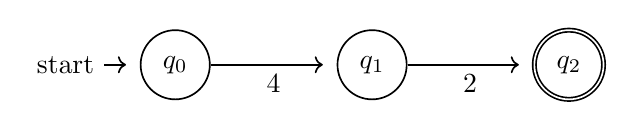
\begin{tikzpicture}[->,
    shorten >=5pt,
    node distance=2.5cm,
    semithick]
    \node[initial,state] (R) {$q_0$};
    \node[state] (S) [right of=R] {$q_1$};
    \node[state,accepting] (T) [right of=S] {$q_2$};
    \path (R) edge node [below] {4} (S)
            (S) edge node [below] {2} (T);
\end{tikzpicture}
\end{center}

\begin{flushleft}
    Formal ist dieser Automat wie folgt definiert:
    \begin{align}
        A &= (\Sigma,Q,\delta,q_0,F) \\
        \Sigma &= \{4,2\} \\
        Q &= \{q_0,q_1,q_2\} \\
        \delta &= \{\langle \langle q_0, 4 \rangle, q_1 \rangle, \langle \langle q_1, 2 \rangle, q_2 \rangle \} \\
        F &= \{q_2\}
    \end{align}
    Die Zustände dieses Automaten lassen sich auch etwas anschaulicher in einer Übergangstabelle darstellen:
\end{flushleft}

\begin{center}
\begin{tabular}{|c|c|c|}
    \hline
    $\delta$ & 4 & 2 \\
    \hline
    $q_0$ & $q_1$ & $q_0$ \\
    \hline
    $q_1$ & $q_1$ & $q_2$ \\
    \hline
    $q_2$ & $q_2$ & $q_2$ \\
    \hline
\end{tabular}
\end{center}

\subsection{Mealy Automaten}
\begin{flushleft}
    Mealy-Automaten können im Gegensatz zu normalen endlichen Automaten auch Ausgaben produzieren.
    Ein normaler endlicher Automat (Akzeptor) kann nur Eingaben akzeptieren oder ablehnen.
    Deshalb sind Mealy-Automaten etwas komplizierter als Akzeptoren, sie werden in der Regel durch einen 7er-Tupel definiert:
    \begin{align}
        A=(\Sigma,\Omega,Q,\delta,\lambda,q_0,F)
    \end{align}
    Neu sind hier bloß $\Omega$, die Menge der Ausgabesymbole und $\lambda: Q \times \Sigma \rightarrow \Omega$, die Ausgabefunktion.
\end{flushleft}

\subsection{Potenzmengenkonstruktion}
\begin{flushleft}
    Die Funktionsweise von deterministischen endlichen Automaten lässt sich relativ einfach erkennen.
    Bei nicht-deterministischen endlichen Automaten ist das aber nicht so, deshalb kann man eine Potenzmengenkonstruktion 
    durchführen um einen beliebigen nicht-deterministischen endlichen Automaten (NEA) in einen deterministischen endlichen 
    Automaten (DEA) umzuwandeln.
    \subsubsection{Beispiel \cite{potenzmengenkonstruktion}}
    Dieser NEA soll jetzt beispielhaft in einen DEA umgewandelt werden:
\end{flushleft}
    
\begin{center}
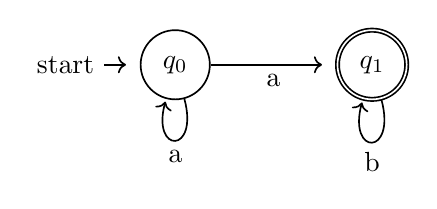
\begin{tikzpicture}[->,
    shorten >=5pt,
    node distance=2.5cm,
    semithick]
    \node[initial,state] (R) {$q_0$};
    \node[state,accepting] (S) [right of=R] {$q_1$};
    \path (R) edge [loop below,below] node {a} (R)
            (R) edge [below] node {a} (S)
            (S) edge [loop below,below] node {b} (S);
\end{tikzpicture}
\end{center}

\begin{flushleft}
    Der erste Schritt ist hierbei das Bestimmen der Zustandsmenge $Q$. In diesem Beispiel gilt:
    \begin{align}
        Q=\{q_0,q_1\}
    \end{align}
    Um nun einen DEA aus diesem NEA zu machen muss die Potenzmenge dieser Zustandsmenge bestimmt werden.
    Dieser Prozess könnte bereits aus der Mengenlehre bekannt sein, $Q'$ ist hier die Potenzmenge von $Q$:
    \begin{align}
        Q &=\{q_0,q_1\} \\
        Q' &=\{\emptyset,\{q_0\},\{q_1\},\{q_0,q_1\}\}
    \end{align}
    Das Symbol $\emptyset$ steht für die leere Menge $\{\}$. Diese Potenzmenge $Q'$ ist die Zustandsmenge 
    des neuen DEA. Um später einen schöneren Übergangsgraph zeichnen zu können wird diese Menge $Q'$ vereinfacht:
    \begin{align}
        Q'' =\{\emptyset,q_0,q_1,q_{01}\}
    \end{align}
    Wichtig zu beachten ist, dass $q_1 \neq q_{01}$ ist, da $q_1=\{q_1\}$ und $q_{01}=\{q_0,q_1\}$ ist.
    Mit der Menge $Q''$ als Zustandsmenge unseres DEA, sieht der erste Entwurf des Übergangsgraphen etwa so aus:
\end{flushleft}
    
\begin{center}
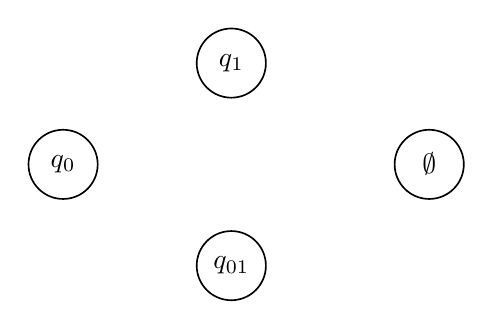
\begin{tikzpicture}[->,
    shorten >=5pt,
    node distance=2.5cm,
    semithick]
    \node[state] (0) {$q_0$};
    \node[state] (1) [above right=0.65cm and 1.5cm of 0] {$q_1$};
    \node[state] (2) [below right=0.65cm and 1.5cm of 0] {$q_{01}$};
    \node[state] (E) [right=3.75cm of 0] {$\emptyset$};
\end{tikzpicture}
\end{center}

\begin{flushleft}
    Wir beginnen damit die Start- und Endzustände zu bestimmen. Den Startzustand (hier $q_0$) können 
    wir einfach übernehmen. Bei den Endzuständen ist das Vorgehen etwas anders, jeder Zustand, dessen Menge 
    einen Endzustand des NEA enthält ist ein Endzustand des DEA. In diesem Beispiel sind also $q_1$ und $q_{01}$
    Endzustände:
\end{flushleft}
    
\begin{center}
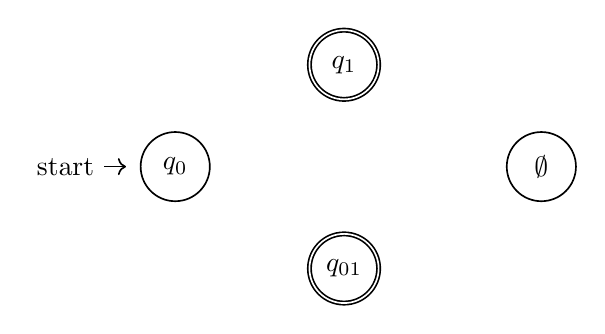
\begin{tikzpicture}[->,
    shorten >=5pt,
    node distance=2.5cm,
    semithick]
    \node[initial,state] (0) {$q_0$};
    \node[accepting,state] (1) [above right=0.65cm and 1.5cm of 0] {$q_1$};
    \node[accepting,state] (2) [below right=0.65cm and 1.5cm of 0] {$q_{01}$};
    \node[state] (E) [right=3.75cm of 0] {$\emptyset$};
\end{tikzpicture}
\end{center}

\begin{flushleft}
    Um die Übergänge des DEA zu bestimmen, zeichnen wir zu erst die Übergangstabelle des NEA:
\end{flushleft}
    
\begin{center}
\begin{tabular}{|c|c|c|}
    \hline
    $\delta$ & a & b \\
    \hline
    $q_0$ & $\{q_0,q_1\}$ & $\emptyset$ \\
    \hline
    $q_1$ & $\emptyset$ & $q_1$ \\
    \hline
    $\emptyset$ & $\emptyset$ & $\emptyset$ \\
    \hline
\end{tabular}
\end{center}

\begin{flushleft}
    Hier ist relativ leicht zu erkennen, dass $\{q_0,q_1\}$ der Grund für den fehlenden 
    Determinismus des NEA ist. Genau dieser Ausdruck sollte uns jedoch aus der vereinfachten Potenzmenge 
    $Q''$ bekannt vorkommen, $\{q_0,q_1\}=q_{01}$. Um einen DEA aus dem NEA zu machen muss man hier also bloß 
    $\{q_0,q_1\}$ durch den neuen Zustand $q_{01}$ austauschen:
\end{flushleft}
    
\begin{center}
\begin{tabular}{|c|c|c|}
    \hline
    $\delta$ & a & b \\
    \hline
    $q_0$ & $q_{01}$ & $\emptyset$ \\
    \hline
    $q_1$ & $\emptyset$ & $q_1$ \\
    \hline
    $q_{01}$ & ? & ? \\
    \hline
    $\emptyset$ & $\emptyset$ & $\emptyset$ \\
    \hline
\end{tabular}
\end{center}

\begin{flushleft}
    Um einen kompletten DEA zu konstruieren muss jedoch noch definiert werden, wie sich der DEA bei $q_{01}$ verhält.
    Dieses Verhalten muss aus dem NEA genommen werden. Da $q_{01}$ die Menge von $q_0$ und $q_1$ ist, kombiniert $q_{01}$
    das Verhalten dieser beiden Zustände. Bei einem $a$ bleibt der DEA also im Zustand $q_{01}$ und bei einem $b$ wandert 
    der DEA in den Zustand $q_1$:
\end{flushleft}

\begin{center}
\begin{tabular}{|c|c|c|}
    \hline
    $\delta$ & a & b \\
    \hline
    $q_0$ & $q_{01}$ & $\emptyset$ \\
    \hline
    $q_1$ & $\emptyset$ & $q_1$ \\
    \hline
    $q_{01}$ & $q_{01}$ & $q_1$ \\
    \hline
    $\emptyset$ & $\emptyset$ & $\emptyset$ \\
    \hline
\end{tabular}
\end{center}

\begin{flushleft}
    Basierend auf dieser Übergangstabelle kann man diesen Übergangsgraphen zeichnen:
\end{flushleft}

\begin{center}
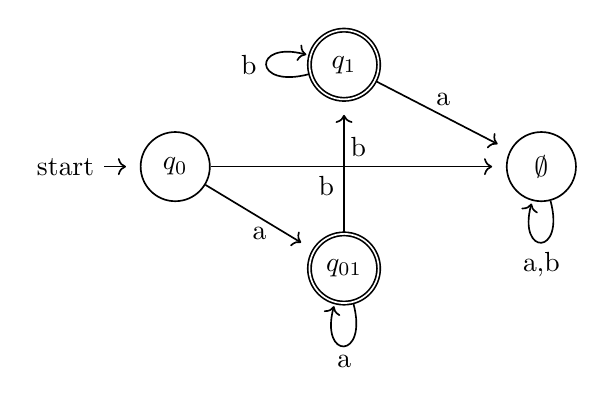
\begin{tikzpicture}[->,
    shorten >=5pt,
    node distance=2.5cm,
    semithick]
    \node[initial,state] (0) {$q_0$};
    \node[accepting,state] (1) [above right=0.65cm and 1.5cm of 0] {$q_1$};
    \node[accepting,state] (2) [below right=0.65cm and 1.5cm of 0] {$q_{01}$};
    \node[state] (E) [right=3.75cm of 0] {$\emptyset$};
    \path (0) edge [below] node {a} (2)
            (0) edge [above] node {b} (E)
            (1) edge [above] node {a} (E)
            (1) edge [loop left] node {b} (1)
            (2) edge [loop below] node {a} (2)
            (2) edge [below left] node {b} (1)
            (E) edge [loop below] node {a,b} (E);
\end{tikzpicture}
\end{center}

\begin{flushleft}
    Um diesen unordentlichen Graphen zu bereinigen kann man hier den sogenannten Papierkorbzustand $\emptyset$
    entfernen. Die Übergangstabelle würde dann so aussehen:
\end{flushleft}

\begin{center}
\begin{tabular}{|c|c|c|}
    \hline
    $\delta$ & a & b \\
    \hline
    $q_0$ & $q_{01}$ & $q_0$ \\
    \hline
    $q_1$ & $q_1$ & $q_1$ \\
    \hline
    $q_{01}$ & $q_{01}$ & $q_1$ \\
    \hline
\end{tabular}
\end{center}

\begin{flushleft}   
    Hier der übersichtliche Übergangsgraph:
\end{flushleft}

\begin{center}
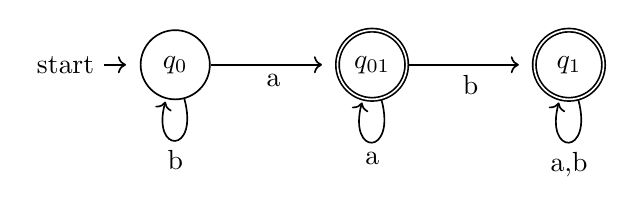
\begin{tikzpicture}[->,
    shorten >=5pt,
    node distance=2.5cm,
    semithick]
    \node[initial,state] (0) {$q_0$};
    \node[accepting,state] (2) [right of=0] {$q_{01}$};
    \node[accepting,state] (1) [right of=2] {$q_1$};
    \path (0) edge [below] node {a} (2)
        (0) edge [loop below] node {b} (0)
        (1) edge [loop below] node {a,b} (1)
        (2) edge [loop below] node {a} (2)
        (2) edge [below] node {b} (1);
\end{tikzpicture}
\end{center}

\subsection{Programmierung von DEA's}
\begin{flushleft}
    Es gibt natürlich verschiedene Wege DEA's zu programmieren, hier gehe ich jedoch nur auf einen Weg ein,
    der grundlegend für jeden DEA funktioniert. Dieser Weg erfordert jedoch auch abhängig von der Komplexität des DEA's
    ein komplexeres Programm.
\end{flushleft}

\begin{flushleft}
    Bei der Simulation eines DEA's ist es eigentlich am wichtigsten zu wissen, ob ein bestimmtes Wort von dem DEA akzeptiert oder
    abgelehnt wird. Man fragt sich also ob der Zustand, der am Ende eines Wortes erreicht wird ein Endzustand ist.
    Um diese Frage zu beantworten braucht man zunächst einen Weg den jetzigen Zustand zu speichern.
    Dafür kann man einen einfachen Integer nutzen, ein bestimmter Wert des Integers steht dann also für einen bestimmten Zustand des Automaten.
\end{flushleft}

\begin{flushleft}
    Ab hier sollte weiter anhand von einem Beispiel erklärt werden, dafür nutze ich das obrige \nameref{sec:Beispiel} eines DEA,
    der nur das Wort $w_0=42$ akzeptiert.
    Hier noch einmal der Übergangsgraph dieses DEA:
\end{flushleft}

\begin{center}
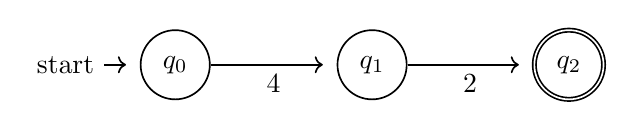
\begin{tikzpicture}[->,
    shorten >=5pt,
    node distance=2.5cm,
    semithick]
    \node[initial,state] (R) {$q_0$};
    \node[state] (S) [right of=R] {$q_1$};
    \node[state,accepting] (T) [right of=S] {$q_2$};
    \path (R) edge node [below] {4} (S)
            (S) edge node [below] {2} (T);
\end{tikzpicture}
\end{center}

\begin{flushleft}
    Hier seine formale Definition:
    \begin{align}
        A &= (\Sigma,Q,\delta,q_0,F) \\
        \Sigma &= \{4,2\} \\
        Q &= \{q_0,q_1,q_2\} \\
        \delta &= \{\langle \langle q_0, 4 \rangle, q_1 \rangle, \langle \langle q_1, 2 \rangle, q_2 \rangle \} \\
        F &= \{q_2\}
    \end{align}
    Für dieses Beispiel sollte unser Integer im Programmcode drei verschiedene Werte annehmen können,
    die Menge $I$ enthält diese Werte:
    \begin{align}
        I=\{0,1,2\}
    \end{align}
    Ein Wert steht immer für einen Zustand, $0$ steht hier also für $q_0$.
    Zunächst erstellen wir die Klasse \textit{Automat}, die das Verhalten des DEA simulieren soll.
    Die Methode \textit{isValid(word)} gibt \textit{true} oder \textit{false} zurück abhängig davon ob der Automat den String \textit{word} akzeptiert oder ablehnt:
\end{flushleft}

\begin{center}  
\begin{lstlisting}
public class Automat {
    // der jetzige Zustand
    private int zustand;

    // Gibt zurueck ob der String "word" akzeptiert wird.
    public boolean isValid(String word) {
        // TODO
    }
}
\end{lstlisting}
\href{https://raw.githubusercontent.com/tim-tm/articles/refs/heads/main/informatik-notes/code/Automat.java}{\textit{Unkommentierter Code}} \\
\end{center}

\begin{flushleft}
    Ein Automat verarbeitet jedes Zeichen eines Wortes nacheinander, das sollte unser Programm auch so machen.
    Es gibt natürlich verschiedene Wege dies in Java umzusetzen, ich persönlich nutze jedoch gerne foreach-Schleifen,
    deshalb wird der String \textit{word} erst in ein char-Array umgewandelt:
\end{flushleft}

\begin{center}
\begin{lstlisting}
public class Automat {
    // der jetzige Zustand
    private int zustand;

    // Gibt zurueck ob der String "word" akzeptiert wird.
    public boolean isValid(String word) {
        // String --> char[]
        char[] arr = word.toCharArray();

        // jeden char in "word" bearbeiten
        for (char c : arr) {
            // ...
        }
    }
}
\end{lstlisting}
\href{https://raw.githubusercontent.com/tim-tm/articles/refs/heads/main/informatik-notes/code/Automat.java}{\textit{Unkommentierter Code}} \\
\end{center}

\begin{flushleft}
    Jetzt geht es darum das Verhalten des Automaten zu simulieren, also erstellen wir ein switch-case Statement mit einem case für
    jeden bekannten Wert des Integers:
\end{flushleft}

\begin{center}
\begin{lstlisting}
public class Automat {
    // der jetzige Zustand
    private int zustand;

    // Gibt zurueck ob der String "word" akzeptiert wird.
    public boolean isValid(String word) {
        // String --> char[]
        char[] arr = word.toCharArray();

        // jeden char in "word" bearbeiten
        for (char c : arr) {
            switch (zustand) {
                case 0: {
                    // verhalten im ersten Zustand
                    break;
                }
                case 1: {
                    // verhalten im zweiten Zustand
                    break;
                }
                case 2: {
                    // verhalten im dritten Zustand
                    break;
                }
            }
        }
    }
}
\end{lstlisting}
\href{https://raw.githubusercontent.com/tim-tm/articles/refs/heads/main/informatik-notes/code/Automat.java}{\textit{Unkommentierter Code}} \\
\end{center}

\begin{flushleft}
    Jetzt kopieren wir das Verhalten jedes Zustands:
\end{flushleft}

\begin{center}
\begin{lstlisting}
public class Automat {
    // der jetzige Zustand
    private int zustand;

    // Gibt zurueck ob der String "word" akzeptiert wird.
    public boolean isValid(String word) {
        // String --> char[]
        char[] arr = word.toCharArray();

        // jeden char in "word" bearbeiten
        for (char c : arr) {
            switch (zustand) {
                case 0: {
                    if (c == '4') {
                        zustand = 1;
                    }
                    break;
                }
                case 1: {
                    if (c == '2') {
                        zustand = 2;
                    }
                    break;
                }
                // case 2 entfernt, da der Zustand q2 keinen Uebergang hat
            }
        }
    }
}
\end{lstlisting}
\href{https://raw.githubusercontent.com/tim-tm/articles/refs/heads/main/informatik-notes/code/Automat.java}{\textit{Unkommentierter Code}} \\
\end{center}

\begin{flushleft}
    Die Zustandsvariable wird verändert, \textit{isValid} gibt aber noch nicht aus ob der Automat akzeptiert oder nicht.
    Dafür kann man einfach abfragen ob die Zustandsvariable den Wert 2 hat, da $q_2$ ein Endzustand ist:
\end{flushleft}

\begin{center}
\begin{lstlisting}
public class Automat {
    // der jetzige Zustand
    private int zustand;

    // Gibt zurueck ob der String "word" akzeptiert wird.
    public boolean isValid(String word) {
        // String --> char[]
        char[] arr = word.toCharArray();

        // jeden char in "word" bearbeiten
        for (char c : arr) {
            switch (zustand) {
                case 0: {
                    if (c == '4') {
                        zustand = 1;
                    }
                    break;
                }
                case 1: {
                    if (c == '2') {
                        zustand = 2;
                    }
                    break;
                }
                // case 2 entfernt, da der Zustand q2 keinen Uebergang hat
            }
        }

        if (zustand == 2) {
            return true;
        } else {
            return false;
        }
    }
}
\end{lstlisting}
\href{https://raw.githubusercontent.com/tim-tm/articles/refs/heads/main/informatik-notes/code/Automat.java}{\textit{Unkommentierter Code}} \\
\end{center}

\begin{flushleft}
    Hier kann die if-Abfrage vereinfacht werden: 
\end{flushleft}

\begin{center}
\begin{lstlisting}
public class Automat {
    // der jetzige Zustand
    private int zustand;

    // Gibt zurueck ob der String "word" akzeptiert wird.
    public boolean isValid(String word) {
        // String --> char[]
        char[] arr = word.toCharArray();

        // jeden char in "word" bearbeiten
        for (char c : arr) {
            switch (zustand) {
                case 0: {
                    if (c == '4') {
                        zustand = 1;
                    }
                    break;
                }
                case 1: {
                    if (c == '2') {
                        zustand = 2;
                    }
                    break;
                }
                // case 2 entfernt, da der Zustand q2 keinen Uebergang hat
            }
        }

        return zustand == 2;
    }
}
\end{lstlisting}
\href{https://raw.githubusercontent.com/tim-tm/articles/refs/heads/main/informatik-notes/code/Automat.java}{\textit{Unkommentierter Code}} \\
\end{center}

\begin{flushleft}
    Was passiert aber nun, wenn isValid mehrmals aufgerufen wird?
    Die Zustandsvariable muss beim zweiten Aufruf nicht unbedingt 0 (Startzustand $q_0$) sein,
    deshalb stellen wir sicher, dass die Variable beim Aufruf von \textit{isValid} immer auf 0 gesetzt wird:
\end{flushleft}

\begin{center}
\begin{lstlisting}
public class Automat {
    // der jetzige Zustand
    private int zustand;

    // Gibt zurueck ob der String "word" akzeptiert wird.
    public boolean isValid(String word) {
        // sicherstellen, dass isValid im Startzustand startet
        zustand = 0;

        // String --> char[]
        char[] arr = word.toCharArray();

        // jeden char in "word" bearbeiten
        for (char c : arr) {
            switch (zustand) {
                case 0: {
                    if (c == '4') {
                        zustand = 1;
                    }
                    break;
                }
                case 1: {
                    if (c == '2') {
                        zustand = 2;
                    }
                    break;
                }
                // case 2 entfernt, da der Zustand q2 keinen Uebergang hat
            }
        }

        return zustand == 2;
    }
}
\end{lstlisting}
\href{https://raw.githubusercontent.com/tim-tm/articles/refs/heads/main/informatik-notes/code/Automat.java}{\textit{Unkommentierter Code}} \\
\end{center}

\begin{flushleft}
    Wenn man möchte kann man auch noch eine Methode schreiben, die den jetzigen Zustand zurück gibt:
\end{flushleft}

\begin{center}
\begin{lstlisting}
public class Automat {
    // der jetzige Zustand
    private int zustand;

    // Gibt zurueck ob der String "word" akzeptiert wird.
    public boolean isValid(String word) {
        // sicherstellen, dass isValid im Startzustand startet
        zustand = 0;

        // String --> char[]
        char[] arr = word.toCharArray();

        // jeden char in "word" bearbeiten
        for (char c : arr) {
            switch (zustand) {
                case 0: {
                    if (c == '4') {
                        zustand = 1;
                    }
                    break;
                }
                case 1: {
                    if (c == '2') {
                        zustand = 2;
                    }
                    break;
                }
                // case 2 entfernt, da der Zustand q2 keinen Uebergang hat
            }
        }

        return zustand == 2;
    }

    // gibt den jetzigen Zustand zurueck
    public int getZustand() {
        return zustand;
    }
}
\end{lstlisting}
\href{https://raw.githubusercontent.com/tim-tm/articles/refs/heads/main/informatik-notes/code/Automat.java}{\textit{Unkommentierter Code}} \\
\end{center}

\begin{flushleft}
    Außerdem kann man einen kleinen Test für die \textit{isValid} Methode schreiben:
\end{flushleft}

\begin{center}
\begin{lstlisting}
public static void main(String[] args) {
    // erstelle ein Automat Objekt
    Automat a = new Automat();
    // sollte "true" ausgeben
    System.out.println(a.isValid("42"));
    // sollte "false" ausgeben
    System.out.println(a.isValid("43"));
}
\end{lstlisting}
\href{https://raw.githubusercontent.com/tim-tm/articles/refs/heads/main/informatik-notes/code/Automat.java}{\textit{Unkommentierter Code}} \\
\end{center}


\bibliographystyle{abbrv}
\bibliography{refs}
\end{document}
